\chapter{Commercial Real Estate Brokers Advice To Young People}

This interview is brief, but it unfolds with real order. We begin with advice to a younger self, move through the handling of money, and only then arrive at commercial real estate as a relationship market. The chapter should preserve that progression. Since no validated board images survive for this lecture, the equations and diagrams below are not transcriptions of visible chalkwork; they are cautious reconstructions of the mechanism the speaker lays out in words.

\section{Personal Discipline Before Strategy}

The first question is retrospective: what would one tell the twenty-year-old self? The answer is rough, even comic, but its force is serious. Before there is a market to enter, there is a life to stop wasting. The lecture therefore begins where many commercial stories do not begin: not with opportunity, but with self-command.

That is the right first beat. The later advice is not offered as a trick for getting rich; it is offered as something that becomes available only after distraction has been cut away. The underlying quantity is not yet money, nor even knowledge, but the ability to sustain effort over time.

We may compress the opening movement into the schematic relation
\begin{equation}
\text{discipline} \to \text{sustained effort}.
\end{equation}
This formula is only a guide for the notes, but it captures the lecture's first premise: if effort is scattered, the rest of the chain cannot hold.

\section{Early Money and the Prevention of Waste}

The speaker then makes the moral point concrete. He names the forms of leakage: chasing girls, drinking beer, and then, once money arrives, buying the wrong kind of symbol. The Porsche example matters because it keeps the chapter out of vague sermonizing. The warning is not against making money. The warning is against converting early gains into vanity and drift.

We should therefore distinguish income from retained advantage. A rise in earnings does not by itself license a rise in status consumption:
\begin{equation}
Y \uparrow \not\Rightarrow C_s \uparrow,
\end{equation}
where \(Y\) denotes income and \(C_s\) denotes conspicuous consumption. The point is qualitative, not econometric. The lecture gives us no utility function, no budget constraint, no portfolio theory. What it gives us is sharper: money earned is not yet wealth secured, and wasted attention is as dangerous as wasted cash.

This also explains why the interview begins as it does. The advice to the younger self is not detached from the later career advice. It is its precondition.

\section{Credibility, Seven Figures, and the Choice of Industry}

At exactly this point the interviewer asks the natural test question: how much money did you actually make? The answer is compact but important. ``In the seven digits'' is not a precise number, and we should not force one upon it. The most faithful mathematical rendering is simply
\begin{equation}
10^6 \le Y < 10^7.
\end{equation}

That short numerical claim changes the weight of everything that came before. It turns the warning against waste from moral advice into experienced advice. Only then does the interview ask the next question: what industry produced that result? The answer is commercial real estate.

Now the lecture pivots. We are no longer speaking only about youth, discipline, and consumption. We are speaking about entry into a particular market. The new question is therefore operational: how does one break in?

\section{Commercial Real Estate as a Relationship Market}

The first answer is a governing principle: commercial real estate is relationship-based. This is the lecture's central proposition. It is stated before any tactics are given, and that order matters. We are first told what kind of market this is; only afterward are we told how to move inside it.

A useful notation is the following.

\begin{definition}
Fix a local market \(\mathcal{M}\). Let \(B(\mathcal{M})\) denote the set of buildings relevant to the beginner's chosen territory. Let \(L_t \subseteq B(\mathcal{M})\) denote the buildings or lobbies physically covered by stage \(t\). Let \(A_t\) denote the intensity of active fieldwork at stage \(t\): visits, time in lobbies, follow-up, and repeated circulation through the market. Let \(K_t\) denote the stock of practical local knowledge generated by that coverage, and let \(R_t\) denote the stock of relationships built from repeated, informed contact.
\end{definition}

The speaker's injunction to ``know every building'' should be read relative to \(\mathcal{M}\), not as a literal claim about mastering an entire city at once. In that local sense,
\begin{equation}
L_t \subseteq B(\mathcal{M}), \qquad K_t = K(L_t),
\end{equation}
with the understanding that wider and deeper coverage produces more usable knowledge.

The lecture's conceptual structure can then be pictured as follows.

\begin{figure}
\centering
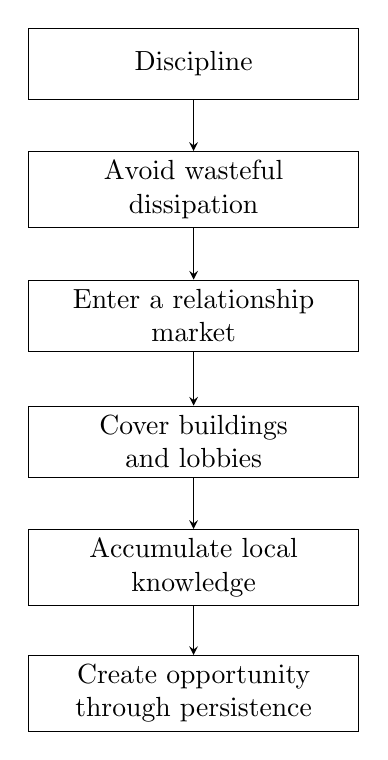
\begin{tikzpicture}[>=stealth]
\node[draw, rectangle, align=center, minimum width=4.2cm, minimum height=0.9cm] (a) at (0,0) {Discipline};
\node[draw, rectangle, align=center, minimum width=4.2cm, minimum height=0.9cm] (b) at (0,-1.6) {Avoid wasteful\\dissipation};
\node[draw, rectangle, align=center, minimum width=4.2cm, minimum height=0.9cm] (c) at (0,-3.2) {Enter a relationship\\market};
\node[draw, rectangle, align=center, minimum width=4.2cm, minimum height=0.9cm] (d) at (0,-4.8) {Cover buildings\\and lobbies};
\node[draw, rectangle, align=center, minimum width=4.2cm, minimum height=0.9cm] (e) at (0,-6.4) {Accumulate local\\knowledge};
\node[draw, rectangle, align=center, minimum width=4.2cm, minimum height=0.9cm] (f) at (0,-8.0) {Create opportunity\\through persistence};

\draw[->] (a) -- (b);
\draw[->] (b) -- (c);
\draw[->] (c) -- (d);
\draw[->] (d) -- (e);
\draw[->] (e) -- (f);
\end{tikzpicture}
\end{figure}

This figure is not evidence from a retained screenshot. It is a transcript-backed map of the lecture's own order of argument.

\subsection{Question \& Answer}

\paragraph{Question.} If the market is relationship-based, what does a beginner actually do? The lecture itself poses this tension. ``Relationships'' is true, but too abstract. If we leave the chapter there, we lose the speaker's main contribution.

\paragraph{Answer.} The abstraction is immediately resolved by physical instruction. Know every building. Be in the lobby of every building. Figure out what is going on there. The speaker does not treat relationships as detachable social capital floating free of place. He treats them as something generated by repeated presence inside a concrete market.

The answer can therefore be written as a process rather than a slogan:
\begin{equation}
\text{coverage} + \text{presence} + \text{local knowledge} \to \text{relationship}.
\end{equation}
This is the point at which the lecture becomes fully operational.

\section{Territory Coverage as Commercial Method}

Once that question has been answered, the chapter should slow down and let the mechanism unfold. The lecture does not recommend generic networking. It recommends territorial coverage. One goes to the buildings, stands in their lobbies, observes, asks, and learns what is happening. The business logic is cumulative.

A restrained update model is
\begin{align}
K_{t+1} &= K_t + \alpha A_t, \\
R_{t+1} &= R_t + \beta A_t + \gamma K_t,
\end{align}
with \(\alpha,\beta,\gamma > 0\). The first line says that activity raises local knowledge. The second says that relationships are built by activity, but activity becomes more productive once it is informed by knowledge.

We may now give the lecture's mechanism as a worked derivation.

\paragraph{Worked derivation.}
\begin{enumerate}
\item Commercial real estate is introduced as a relationship market.
\item A relationship market does not reward passive interest; it rewards repeated, situated contact.
\item The speaker therefore replaces the abstract command ``build relationships'' with the concrete command ``cover the buildings and stand in the lobbies.''
\item That coverage raises \(K_t\), the stock of local information about who is active, what is moving, and where attention should be placed.
\item Higher \(K_t\) makes each subsequent contact more intelligent, and intelligent contact raises \(R_t\).
\item Thus field activity compounds: what begins as motion becomes information, and what becomes information can become relationship.
\end{enumerate}

We should notice how tight the transcript is at this stage. First comes the claim that the market is relationship-based. Then comes the question of what that means for the beginner. Then comes the answer: cover the territory until the market begins to disclose itself.

\begin{remark}
These update rules are not quoted formulas. They are a careful formal compression of the speaker's method. The notes should keep that status visible.
\end{remark}

\section{Opportunity, Refusal, and the Final Maxim}

Only after the mechanism has been laid out do we reach the final pair of claims: being busy creates opportunity, and one should not take no for an answer. They should be written as consequences of the previous section, not as detached motivational slogans.

Let \(O_t\) denote the flow of opportunities available at stage \(t\). The transcript suggests the monotone dependence
\begin{equation}
O_t = f(K_t,R_t), \qquad \frac{\partial f}{\partial K} > 0, \qquad \frac{\partial f}{\partial R} > 0.
\end{equation}
The meaning is simple. If we know more about the market and are better connected to it, we increase the chance that useful openings appear.

The second maxim concerns refusal. Let \(N_t\) denote a negative response at stage \(t\). Then the operational rule of the lecture is not
\[
N_t = 1 \Longrightarrow A_{t+1} = 0.
\]
It is rather
\begin{equation}
N_t = 1 \Longrightarrow A_{t+1} \ge A_t,
\end{equation}
or at least that activity should continue in redirected form. A rejection closes one path; it does not invalidate the search.

We can now collect the whole movement of the lecture into one final chain:
\begin{equation}
\text{discipline} \to A_t \to K_t \to R_t \to O_t.
\end{equation}
This is the chapter's strongest mathematical summary. It begins with self-command, not with technique, because that is how the lecture itself unfolds.

\section{Summary}

The interview moves in a strict order, and the notes should keep that order visible. First we are told to get serious. Then we are warned not to convert early money into waste. Then the speaker's own success is established by the seven-figure remark. Only after that are we told the industry and the method.

That method is clear. Commercial real estate is treated as a relationship market, but relationships are not introduced as a vague social ideal. They are built by covering a local market, standing in the lobbies, learning what is happening, and returning often enough that information hardens into contact and contact hardens into opportunity. The final maxims therefore land exactly where they should: being busy creates opportunity, and refusal is a reason to continue, not a reason to disappear.